% small.tex
\documentclass{beamer}
\usetheme{Boadilla}
\usepackage{graphicx}
\usepackage{wrapfig}
%algorithms and pseudo code
\usepackage{algorithm}
\usepackage[noend]{algpseudocode}
\usepackage{numprint}
\usepackage{subcaption}
\usepackage{media9}
\usepackage{bibentry}
\usepackage[justification=centering]{caption}
\nobibliography*

\setbeamertemplate{bibliography item}[text]
\setbeamertemplate{author in head/foot}{\insertshortauthor}
\setbeamertemplate{navigation symbols}{}

\newcommand{\lenitem}[2][.6\linewidth]{\parbox[t]{#1}{\strut #2\strut}}
\newcommand{\outline}{
  \begin{frame}<beamer>
    \frametitle{Outline}
    \tableofcontents[currentsection]
  \end{frame}
}

\begin{document}

\title[Unstructured Mesh Workflows]
{
Dynamic Load Balancing of Massively Parallel Unstructured Meshes
}
\author{Gerrett Diamond, Cameron W. Smith, Mark S. Shephard}
%\email{diamog@rpi.edu}
%\author[smithc11@rpi.edu]{Cameron W. Smith\\
%  \smallskip
%  Committee:\\
%  Mark Shephard\\
%  Max Bloomfield, Christopher Carothers, Barbara Cutler, Onkar Sahni
%}

\institute[SCOREC]{
Scientific Computation Research Center \\
Rensselaer Polytechnic Institute
}

\date{November 13, 2017}

%----------- titlepage ----------------------------------------------%
\begin{frame}[plain]
  \titlepage
\end{frame}

%----------- outline ----------------------------------------------%
\begin{frame}
  \frametitle{Outline}
  \tableofcontents
\end{frame}

%----------------------------------------------------------------------%
%----------- Section --------------------------------------------------%
%----------------------------------------------------------------------%
\section{Partitioning and Load Balancing}
\begin{frame}
  \frametitle{Motivation}
  Many evolving distributed simulations have: \\
  \begin{itemize}
    \item Complex relational structures.
    \item Irregular forms of computational and communication costs.
    \item Evolving imbalance of work. %Define Imbalance
    \item Multiple criteria that need balancing simultaneously.
  \end{itemize}
\end{frame}

\begin{frame}
  \frametitle{Common Methods for Partitioning}
  \begin{itemize}
  \item Multilevel Graph Methods %Discuss poor scaling
    \begin{itemize}
    \item ParMETIS
    \item Zoltan
    \end{itemize}
  \item Geometric Methods %Require coordinates
    \begin{itemize}
    \item Recursive Coordinate Bisection (RCB)
    \item Recursive Inertial Bisection (RIB)
    \item Multi-Jagged
    \end{itemize}
  \item Diffusive Methods %Improve a partition efficiently
    \begin{itemize}
    \item Label Propagation
%    \item ParMA
%    \item EnGPar
    \end{itemize}
  \end{itemize}
\end{frame}

%Maybe one more slide to discuss in more detail why we need diffusive load balancing

\section{EnGPar - a graph based diffusive load balancer}

\begin{frame}
  \frametitle{What is EnGPar?}
  \begin{itemize}
  \item A partitioning tool to complement existing multi-level and geometric methods.
  \item Provides a diffusive load balancing algorithm for partition improvement and supports multi-criteria partitioning.
  \item Utilizes a specialized multigraph structure to represent relation based data.
  \item Implemented to support efficient data parallel operations on accelerators and vector units in many core processors.
  \end{itemize}
\end{frame}

\begin{frame}
  \frametitle{Software}
  EnGPar's source can be found at \url{http://scorec.github.io/EnGPar/}.
  \begin{itemize}
  \item Written in C++ using MPI.
  \item Uses PCU for sparse neighborhood exchange peer to peer communications.
  \end{itemize}
\end{frame}

\begin{frame}
  \frametitle{N-graph}
  %EnGPar utilizes an expanded multigraph structure called the N-graph.\\
  %THIS IS TOO MUCH TEXT PROBABLY...
  The N-graph is a multigraph with two modes of operation: traditional or hypergraph.\\
  \smallskip
  The N-graph is defined as the following:
  \begin{itemize}
  \item A set of vertices $V$ representing the atomic units of work.
  \item If using the traditional graph mode:
    \begin{itemize}
    \item $N$ sets of edges $E_0,...,E_{n-1}$ for each type of relation.
    \item Each edge connects two vertices $u,v \in V$.
    \end{itemize}
  \item If using the hypergraph mode:
    \begin{itemize}
    \item $N$ sets of hyperedges $H_0,...,H_{n-1}$ for each type of relation.
    \item $N$ sets of pins $P_0,...,P_{n-1}$ corresponding to each set of hyperedges.
    \item Each pin in $P_i$ connects a vertex, $v \in V$, to a hyperedge $h \in H_i$.
    \end{itemize}
  \end{itemize}
\end{frame}

\begin{frame}
  \frametitle{Mapping structures to the N-graph}
  %Before using EnGPar a simulation must first map its data to the N-graph
  To map to the N-graph simulations must:
  \begin{itemize}
  \item Define units of work as the vertices.
  \item Decide on the mode of edges to use.
  \item Create (hyper)edges between the vertices whose corresponding work relate to each other.
  \end{itemize}
\end{frame}
\begin{frame}
  \frametitle{Mapping structures to the N-graph}

  %Figure showing the conversion from mesh to N-graph
  \begin{figure}
    \centering
    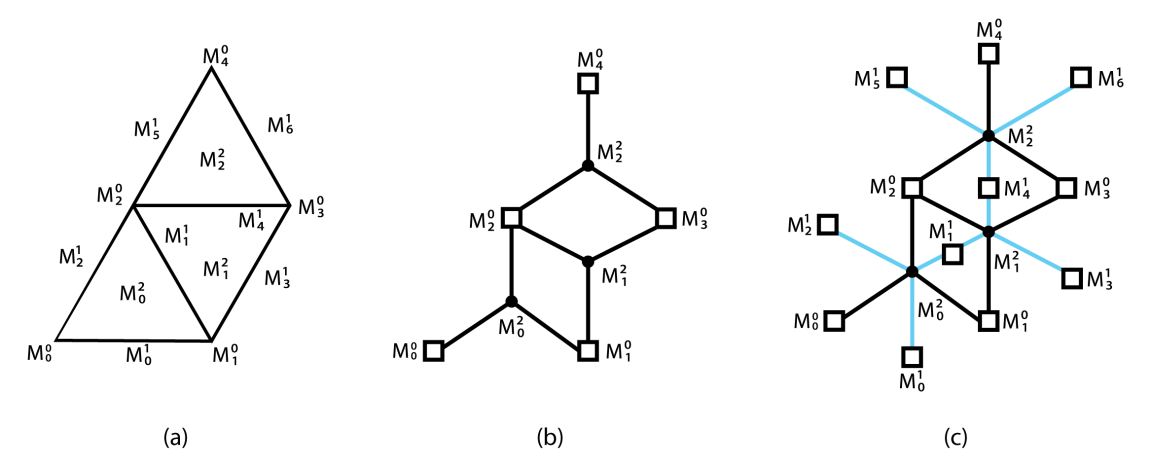
\includegraphics[width=.9\textwidth]{figures/exampleMesh2Graph.png}
    \caption{Converting a triangular mesh(a) to the N-graph with an edge type for mesh vertices (b) and an additional edge type for mesh edges (c).}
  \end{figure}
\end{frame}

\begin{frame}
  \frametitle{Diffusive Terminology}
  \begin{minipage}{0.45\textwidth}
  \begin{itemize}
  \item Sides
    \begin{itemize}
    \item Each part determines which parts are its neighbors.
    \item Determines a measurement of the area between each part.
    \end{itemize}
  \item Cavity
    \begin{itemize}
    \item Defined by (hyper)edges that cross a part boundary.
    \item Includes all the vertices that bound the (hyper)edge.
    \end{itemize}
  \end{itemize}
  \end{minipage} \hfill
  \begin{minipage}{0.5\textwidth}
  \begin{figure}
    \centering
    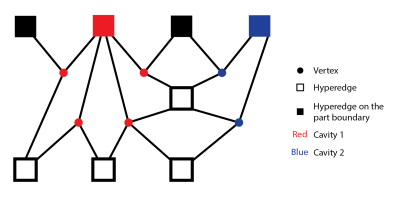
\includegraphics[width=\textwidth]{figures/PartBoundary.png}
    \caption{Two parts of an N-graph with a side of size 4. Two cavities are shown in red and blue for part 0.}
  \end{figure}
  \end{minipage}
\end{frame}
\begin{frame}
  \frametitle{Diffusive Terminology}
  \begin{itemize}
  \item Weights
    \begin{itemize}
    \item Each part computes its weight of the current target entity types, $w_i$.
    \item This weight is shared with all of the part's neighbors(sides).
    \end{itemize}
  \item Targets
    \begin{itemize}
    \item The neighbors that the part will send weight to.
    \item A part, $i$, will send weight to a neighbor, $j$, if:
      \begin{itemize}
      \item $w_i>w_j$
      \item the area between the parts ($s_{ij}$) is less than the average of all part boundaries.  
      \end{itemize}
    \item Weight to send from part $i$ to part $j$ is $\alpha(w_i-w_j)*\dfrac{\text{size}(s_{ij})}{\text{size}(s)}$
      \begin{itemize}
        \item $\alpha$ is an input parameter that limits how much weight is sent in each iteration.
      \end{itemize}
    \end{itemize}
  \end{itemize}
\end{frame}

\begin{frame}
  \frametitle{Diffusive Partitioning}
  \begin{algorithm}[H]
    \caption{Diffusive Load Balancing Framework}
    \label{alg:engpar}
    \small
    \begin{algorithmic}[1]
      \Procedure{Balance}{$ngraph$,$entity\_types$}
      \ForAll{$t \in entity\_types$}
      \While{imbalance of $t >$ tolerance}
      \Call{RunStep}{$ngraph$,$t$}
      \If{Balancing Stagnates}
      \State break
      \EndIf
      \EndWhile
      \EndFor
      \EndProcedure

      \Procedure{RunStep}{$ngraph$,$t$}
      \State $sides = makeSides(ngraph)$
      \State $weights = makeWeights(ngraph,sides,t)$
      \State $targets = makeTargets(ngraph,sides,weights)$
      \State $queue = makeTraversalQueue(ngraph)$
      \State $plan = select(ngraph,targets,queue)$
      \State $ngraph.migrate(plan)$
      \EndProcedure
    \end{algorithmic}
  \end{algorithm}
\end{frame}

\begin{frame}
  \frametitle{Traversal Queue}
  The traversal queue provides an ordering of the (hyper)edges on the part boundary for selection.\\
  \bigskip
  This is done in two steps:
  \begin{itemize}
  \item A breadth-first traversal starting at the part boundary to determine the furthest (hyper)edges as the center of the part.
  \item A breadth-first traversal starting at the center (hyper)edges to compute topological distance for each (hyper)edge on the part boundary.
  \end{itemize}
\end{frame}

\begin{frame}
  \frametitle{Traversal Queue}
  This ordering becomes more difficult to compute when a part is not fully connected. \\
  
  \bigskip
  In this case, centers and distances are calculated separately for each component. \\
  
  \bigskip
  Each disconnected component is ordered from shallowest to deepest.
\end{frame}

\begin{frame}
  \frametitle{Traversal Queue}
  \begin{figure}
    \centering
    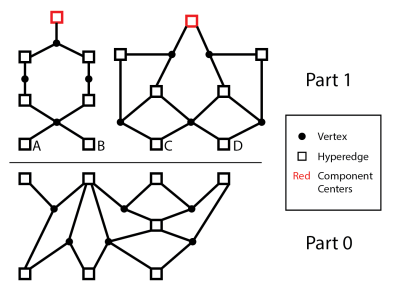
\includegraphics[width=.7\textwidth]{figures/Disconnected.png}
    \caption{The traversal queue computation for two disconnected components in Part 1. The centers of each component are marked in red. The traversal queue for Part 1 is C,D,A,B}
  \end{figure}
\end{frame}

\begin{frame}
  \frametitle{Selection}
  \begin{minipage}{.5\textwidth}
    \begin{itemize}
    \item Iterates over (hyper)edges that cross a part boundary.
      
    \item The cavity defined by the (hyper)edge is chosen for migration if:
      \begin{itemize}
      \item The part that the (hyper)edge is shared with is a target part.
      \item The target part has not been sent more weight than the limit.
      \item The size of the cavity is small.
      \end{itemize}
    \end{itemize}
  \end{minipage}
  \begin{minipage}{.45\textwidth}

    \begin{figure}
      \centering
      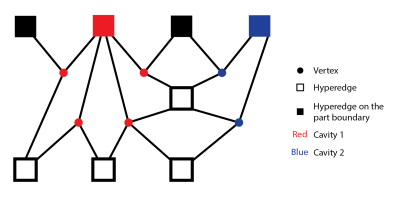
\includegraphics[width=\textwidth]{figures/PartBoundary.png}
    \end{figure}
  \end{minipage}
\end{frame}


\section{Comparison to ParMA}

\begin{frame}
  \frametitle{Problem Setup}
  We compare EnGPar's performance to its predecessor ParMA, which is built to operate directly on unstructured meshes.\\
  \medskip
  ParMA and EnGPar are set to balance a mesh for a finite element analysis where:
  \begin{itemize}
  \item Scalability of matrix formation is sensitive to mesh element imbalance.
  \item Linear algebra routines are sensitive to the imbalance of degrees of freedom.
  \item For this we assume the degrees of freedom are associated with mesh vertices.
  \end{itemize}
  \bigskip
  To partition for this, both balance mesh vertices followed by elements with a target imbalance of 1.05. \\
  
\end{frame}

\begin{frame}
  \frametitle{Problem Setup}
  %Describe the mesh, system run on, initial partition etc.
  \medskip
  Tests were run on a billion element mesh. \\
  \medskip
  Initial partitions are built using:
  \begin{itemize}
  \item Global ParMETIS part k-way to 8Ki($8*2^{10}$) parts.
  \item Local ParMETIS part k-way from 8Ki to 128Ki, 256Ki, and 512Ki parts.
  \end{itemize}
  The partitions before using EnGPar or ParMA are as such:\\
  \begin{table}[!h]
    \centering
    \begin{tabular}{||c|c|c|c||}
      \hline
      Number of Parts &128Ki&256Ki&512Ki \\
      \hline
      Elements per part & 9,836 & 4,918&2,459  \\
      \hline
      Vertex imbalance & 1.13 & 1.18 & 1.53 \\
      \hline
      Element imbalance & 1.02& 1.02& 1.02\\
      \hline
    \end{tabular}
  \end{table}
  All experiments were run on the Mira BlueGene/Q system with one process per hardware thread.
\end{frame}

%More slides to go over the results in the paper
\begin{frame}
  \frametitle{Mesh Vertex Imbalance}
  %Figure showing the conversion from mesh to N-graph
  \begin{figure}
    \centering
    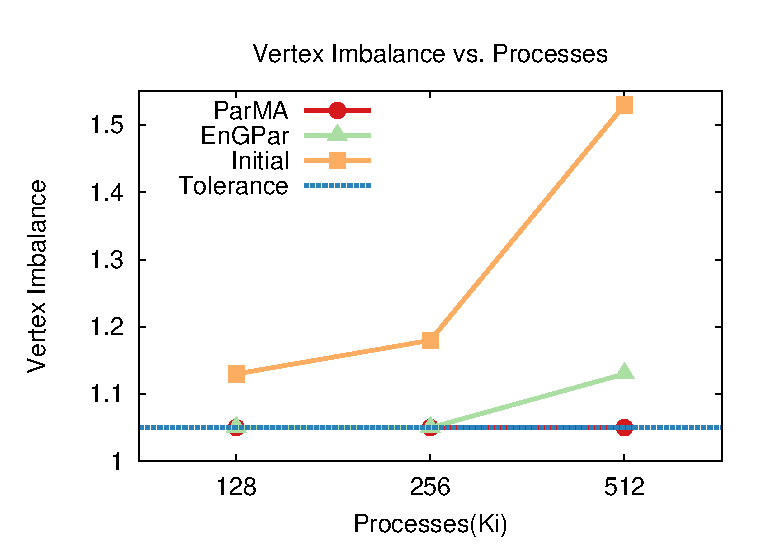
\includegraphics[width=.8\textwidth]{figures/vimb_v_cores.eps}
  \end{figure}  
\end{frame}

\begin{frame}
  \frametitle{Mesh Element Imbalance}
  %Figure showing the conversion from mesh to N-graph
  \begin{figure}
    \centering
    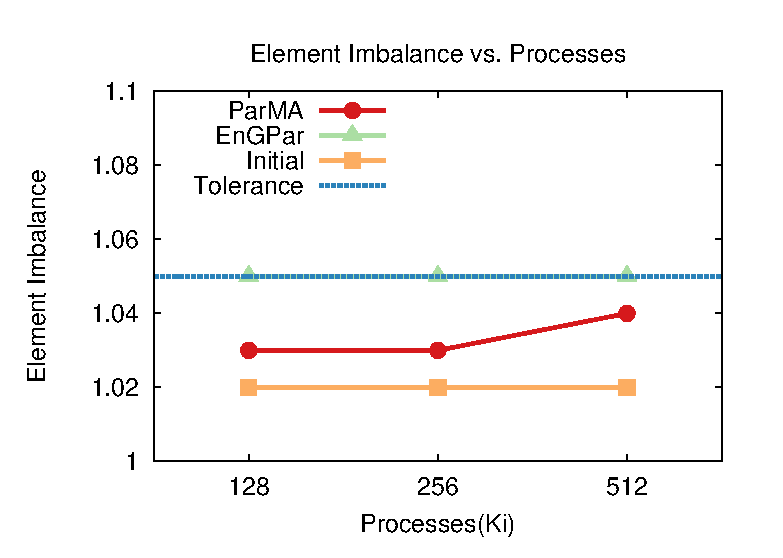
\includegraphics[width=.8\textwidth]{figures/eimb_v_cores.eps}
  \end{figure}  
\end{frame}

\begin{frame}
  \frametitle{RunTime Comparison}
  \begin{figure}
    \centering
    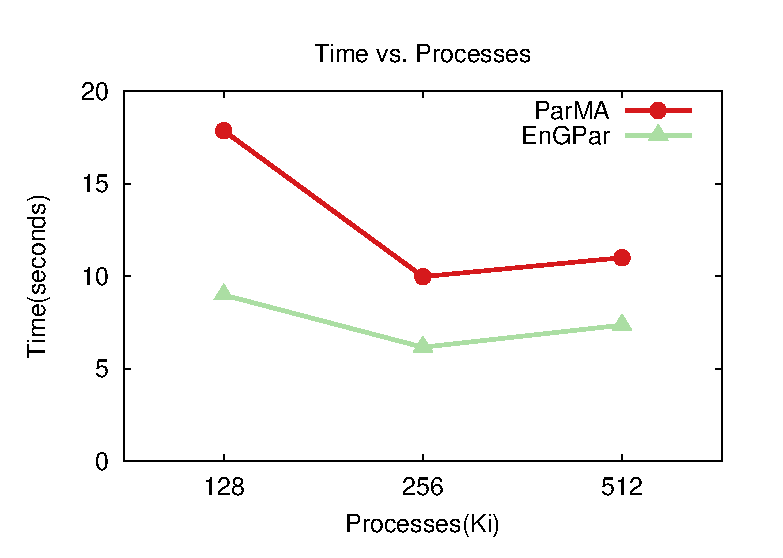
\includegraphics[width=.8\textwidth]{figures/time_v_cores.eps}
  \end{figure}
  
\end{frame}

\begin{frame}
  \frametitle{Future Work}
  Expanding the capabilities of EnGPar:
  \begin{itemize}
  \item Improve partitioning at very high part count.
  \item Improve performance of the balancing procedures using accelerators.
  \end{itemize}
  Applying EnGPar to other applications:
  \begin{itemize}
  \item CODES - a discrete event simulation for communication on supercomputer networks. \url{press3.mcs.anl.gov/codes/}
  \item FUN3D - a computational fluid dynamic simulation using a vertex-based partitioned mesh. \url{fun3d.larc.nasa.gov}
  \item PHASTA - massively parallel computational fluid dynamics. \url{github.com/PHASTA/phasta}
    %For future note: most glorious computational fluid dynamics that scales to the moon...

  \end{itemize}
\end{frame}
  
\end{document}
